\chapter{Simplified RL model}
The models presented in \hyperref[chap:RLModel]{~Chapter \ref*{chap:RLModel}} assume the lick to be a functional action, which is absolutely reasonable in our case because the task presented requires the achievement of the performance criterion both in hit and correct rejection. However, since the obtained reward is solely related to the performance, it possible to build a simplified version of the hybrid Rescorla-Wagner model, without explicitly consider the actions.\\Thus the expected reward values are expressed as follows:
\begin{equation}
V_s(t+1)=V_s(t)+k\cdot\alpha(t)\cdot\delta  \hspace{0.3cm} with \hspace{0.3cm}\delta(t)=r(t)-V_s(t)
\label{VValues}
\end{equation}
where V is now a $
T\times 2$ vector. $\delta$ is again the prediction error. Importantly V values are still modulated according to the time dependent component $\alpha(t)$, related to the uncertainty to get the reward. %The need to introduce a time dependent learning rate was emphasized first in works as \cite{Daw} and \cite{Funamizu}.
In figure \ref{fig:PavRL_ex} is shown an example of, from the top to the bottom, the performance, the reward expectation values $V$, the uncertainty $\alpha$ and the reward prediction error $\delta$.
\begin{figure}
    \centering
    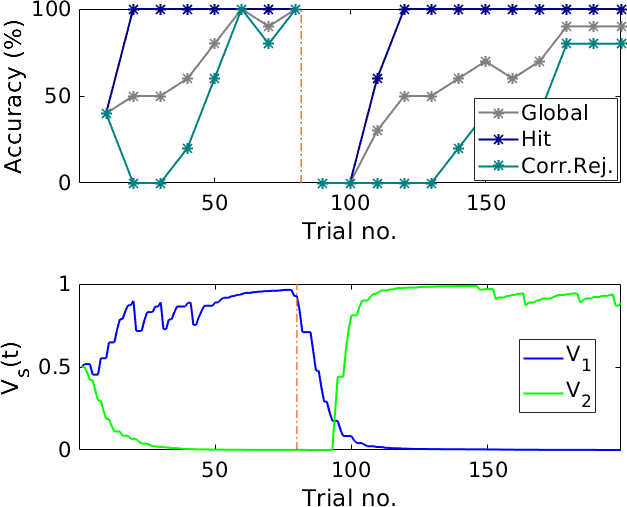
\includegraphics[scale=0.7]{figures/PavPerfV2.png}
    
    \vspace{0.5cm}
    
    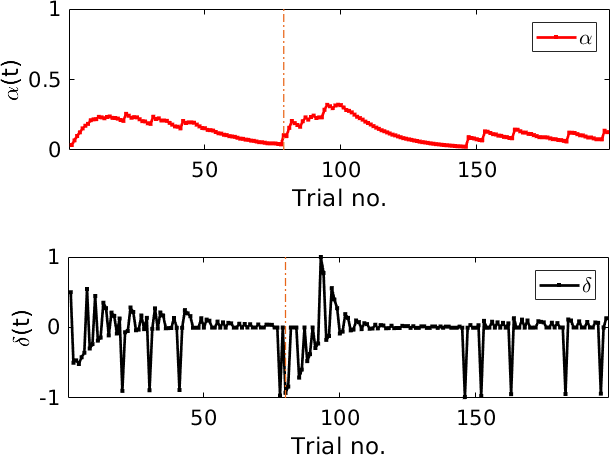
\includegraphics[scale=0.7]{figures/PavAlphaDelta1.png}
    \caption{From the top to the bottom, the animal performance, the reward expectation values $V$, the uncertainty $\alpha$ and the reward prediction error $\delta$.}
    \label{fig:PavRL_ex}
\end{figure}
We tested whether SPN-DAN pairs encode reward prediction error signals using the same argument of \hyperref[sec:Regression]{~Chapter \ref*{sec:Regression}}. If the prediction signal is conveyed by SPN-DAN pairs, their activity must correlate with the certainty, which implies an anticorrelation with the model function $\alpha$, and correlate with prediction error, exemplified by $\delta$ in reinforcement learning models.\\
This hypothesis was tested regressing out $\alpha$ and $\delta$ in two distinct Poisson regression models, where the observations are the SPN-DAN pairs activity. The processes were modeled as follows:
\begin{equation*}
    \log(\mu_t)=\beta_0+\beta\cdot\alpha(t-1)
\end{equation*}
and 
\begin{equation*}
    \log(\mu_t)=\beta_0+\beta\cdot\delta(t)
\end{equation*}
From where $\beta$ parameters are estimated, which inform about correlations between observations and regressors, indicating the percentage variation in observations when the regressor changes of one unit. For detailed discussion see \hyperref[sec:Regression]{~Chapter \ref*{sec:Regression}}.\\
In figure \ref{fig:RL_alphadelta} we show on the left side box plots of standardized regression coefficients $\beta^*$, on the right side empirical cumulative distribution function of $\beta^*$.
\begin{figure}
   \centering
    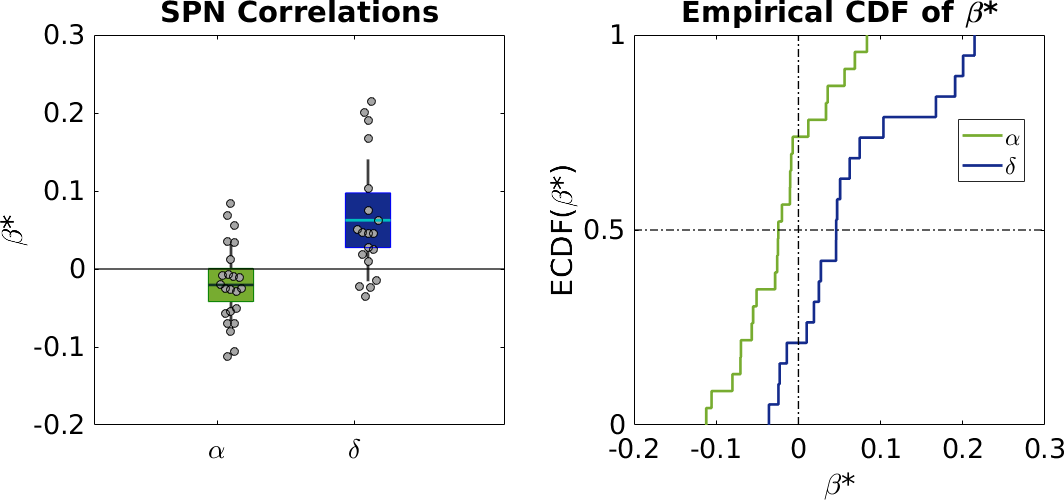
\includegraphics[scale=0.5]{figures/AlphaAndDeltaPavSPN1.png}
    \caption{$\alpha$ and $\delta$ were regressed out in two separated Poisson regression models with the SPN-DAN pairs activity. \textbf{Left:} box plot of standardized regression coefficients $\beta^*$. \textbf{Right:} empirical cumulative distribution function of $\beta^*$}
    \label{fig:RL_alphadelta}
\end{figure}